\documentclass[fleqn,answers,addpoints]{exam}

%\usepackage{graphicx, fancyhdr}
\usepackage{etoolbox}
\usepackage{subcaption}
\usepackage{etoolbox}
\usepackage{tikz,pgfplots}
\usepackage{amsmath, amsfonts}
\usepackage{color}

%% For LaTeX-Box: root = stat105_exam1_info.tex 
%%%%%%%%%%%%%%%%%%%%%%%%%%%%%%%%%%%%%%%%%%%%%%%%%%%%%%%%%%%%%%%%%%%%%%%%%%%%%%%%
%  File Name: stat105_exam1_info.tex
%  Purpose:
%
%  Creation Date: 24-09-2015
%  Last Modified: Thu Sep 24 13:51:36 2015
%  Created By:
%%%%%%%%%%%%%%%%%%%%%%%%%%%%%%%%%%%%%%%%%%%%%%%%%%%%%%%%%%%%%%%%%%%%%%%%%%%%%%%%
\newcommand{\course}[1]{\ifstrempty{#1}{STAT 105}{STAT 105, Section #1}}
\newcommand{\sectionNumber}{B}
\newcommand{\examDate}{October 1, 2015}
\newcommand{\semester}{FALL 2015}
\newcommand{\examNumber}{II}

\newcommand{\examTitle}{Exam \examNumber}

\runningheader{\course{\sectionNumber}}{Exam \examNumber}{\examDate}
\runningfooter{}{}{Page \thepage of \numpages}

\newcommand{\examCoverPage}{
   \begin{coverpages}
   \centering
   {\bfseries\scshape\Huge Exam I \par}
   \vspace{1cm}
   {\bfseries\scshape\LARGE \course{\sectionNumber} \par}
   {\bfseries\scshape\LARGE \semester \par}

   \vspace{2cm}

   \fbox{\fbox{\parbox{5.5in}{\centering 

      \vspace{.25cm} 
      
      {\bfseries\Large Instructions} \\

      \vspace{.5cm} 

      \begin{itemize}
         \item  The exam is scheduled for 80 minutes, from 8:00 to 9:20 AM. At 9:20 AM the exam will end.\\
         \item  A forumula sheet is attached to the end of the exam. Feel free to tear it off.\\
         \item  You may use a calculator during this exam.\\
         \item  Answer the questions in the space provided. If you run out of room, continue on the back of the page. \\
         \item  If you have any questions about, or need clarification on the meaning of an item on this exam, please ask your instructor. No other form of external help is permitted attempting to receive help or provide help to others will be considered cheating.\\
         \item  {\bfseries Do not cheat on this exam.} Academic integrity demands an honest and fair testing environment. Cheating will not be tolerated and will result in an immediate score of 0 on the exam and an incident report will be submitted to the dean's office.\\
      \end{itemize}

   }}}

   \vspace{2cm}

   \makebox[0.6\textwidth]{Name:\enspace\hrulefill}

   \vspace{1cm}

   \makebox[0.6\textwidth]{Student ID:\enspace\hrulefill}
   \end{coverpages}

}


\newcommand{\course}[1]{\ifstrempty{#1}{STAT 305}{STAT 305, Section #1}}
\newcommand{\sectionNumber}{3}
\newcommand{\examDate}{December 14, 2018}
\newcommand{\semester}{Fall 2018}
\newcommand{\examNumber}{}
\newcommand{\qparts}[1]{\begin{parts} #1 \end{parts}}
\newcommand{\qitems}[1]{\begin{itemize} #1 \end{itemize}}

% Document definitions
\newcommand{\examTitle}{\examNumber Final Exam }
\runningheader{\course{\sectionNumber}}{\examNumber Final Exam }{\examDate}
\runningfooter{}{}{Page\ \thepage\ of\ \numpages}

\begin{document}
	
	\begin{coverpages}
		\centering
		{\bfseries\scshape\Huge \examNumber Final Exam  \par}
		\vspace{1cm}
		{\bfseries\scshape\LARGE \course{\sectionNumber} \par}
		{\bfseries\scshape\LARGE \semester \par}
		\vspace{2cm}
		\fbox{\fbox{\parbox{5.5in}{
					\centering 
					\vspace{.25cm} 
					{\bfseries\Large Instructions} \\
					\vspace{.25cm} 
					\begin{itemize}
						\item  The exam is scheduled for 120 minutes, from 12:00 to 2:00pm. At  2:00pm  the exam will end.\\
						\item  A forumula sheet is attached to the end of the exam. Feel free to tear it off.\\
						\item  You are allowed to use a self-produced one-page (front and back) formula sheet during this exam.\\
						\item  You may use a calculator during this exam.\\
						\item  Answer the questions in the space provided. If you run out of room, continue on the back of the page. \\
						\item  If you have any questions about, or need clarification on the meaning of an item on this exam, please ask your instructor. No other form of external help is permitted attempting to receive help or provide help to others will be considered cheating.\\
						\item  {\bfseries Do not cheat on this exam.} Academic integrity demands an honest and fair testing environment. Cheating will not be tolerated and will result in an immediate score of 0 on the exam and an incident report will be submitted to the office of the dean.\\
					\end{itemize}
		}}}
		\vspace{1cm}
		\makebox[0.6\textwidth]{}
		\vspace{1cm}
		\makebox[0.6\textwidth]{Name:\enspace\hrulefill}
		\vspace{1cm}
		\makebox[0.6\textwidth]{Student ID:\enspace\hrulefill}
	\end{coverpages}
	
	\begin{questions}
		
		\question

Portable pneumatic pumps have long been used by hobby machinists, but
are gaining renewed interest as robotics are becoming a more common part
of our daily lives. Specifically, drones can make use of such pumps due
to their weight benefits over hydraulic pumps with equivalent strength.
Amazon is experimenting with using such pumps in its delivery drones and
is interested in factors effecting the lifetime of the pumps.

A team of engineers working for Amazon has been tasked with developing
pumps for delivery drones that improve both time-in-flight (measured in
hours) and the number of pump-actions (the number of times the drone
uses the pump). With those goals in mind, the team designed three pumps:
a single-piston/single-stage design, a dual-piston/single-stage design,
and a dual-piston/dual-stage design. The engineers are testing the pumps
with three types of compressed gas: OFN (oxygen-free nitrogen), Carbon
dioxide, and Oxygen. Concerned about environmental effects, the
engineers selected four locations to test the drones in - San Antonio,
Seattle, Lexington, and Amherst in which to test the drones.

In all four locations they tested the every design-gas combination in
five drones (45 drones in each location). The drones delivered 5 pound
packages from an initial location to a location 2000 meters away,
retrieved the package, and returned it to the original point. The number
of deliveries and the flight time were recorded for each drone.

Note:
\((\text{3 designs}) \cdot (\text{3 gas types}) \cdot (\text{5 drones}) \cdot (\text{4 locations}) = \text{180 total drones}\)

The goal is to determine is to identify how to maximize both flight time
and number of deliveries.

\qparts{
\part[2] Is this an experiment or an observational study? Explain. \vspace{2cm}
\part Identify each of the following and describe them as numeric (in which case, identify whether it is continuous or discrete) or categorcial (in which case list the possible levels). \vspace{1cm}
\begin{subparts}
   \subpart[2] Identify the response variable(s): \vspace{2cm}
   \subpart[2] Identify the experimental variable(s): \vspace{2cm}
   \subpart[2] Blocking variable(s): \vspace{2cm}
\end{subparts}
\part[2] Identify two controlled variables used in this process. \vspace{2cm}
}

\newpage
\question

The quality of a diamond is often described in terms of the four C's: -
carat (the diamonds mass, with 1 carat = 200 milligrams), - cut (a
description of how well the diamond has been shaped), - color (the less
color the more rare), - clarity (a description of the flaws in the
diamond). Of these, carat is the most easily understood in terms of its
impact on the diamonds value: all things being equal, the larger the
diamond the higher its value.

The following plot shows the sale price of 375 diamonds (in thousands of
dollars), which were appraised by experts as having an ideal cut, the
depth, internally flawless clarity, and being colorless or essentially
colorless.

\begin{figure}[h]

{\centering 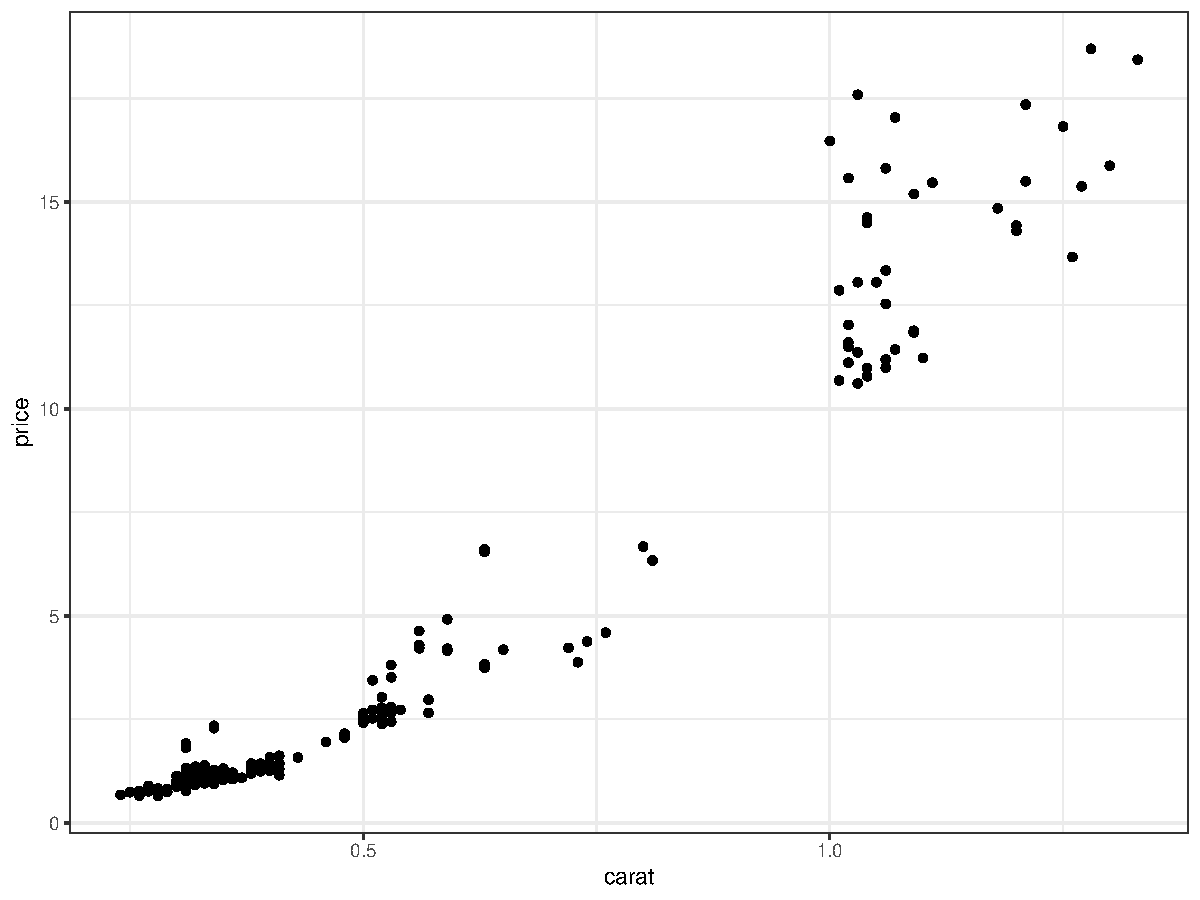
\includegraphics[width=.5\linewidth]{stat305_practice_final_F19_files/figure-latex/unnamed-chunk-3-1} 

}

\caption{Plot depicting the sale price of 375 diamonds with the same quality of cut, clarity, and color. There is a general pattern indicating that higher carat (i.e., the mass) is associated with higher price.}\label{fig:unnamed-chunk-31}
\end{figure}
\begin{figure}[h]

{\centering 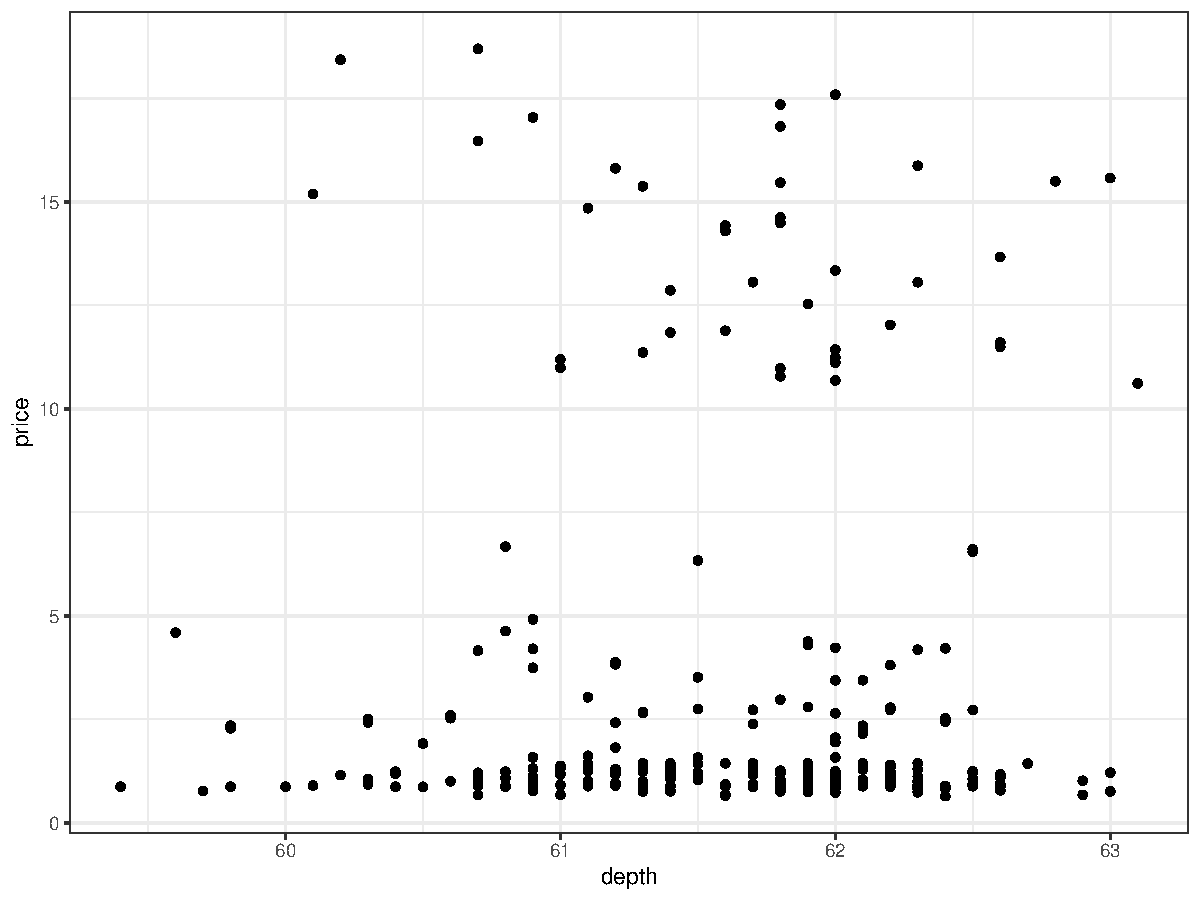
\includegraphics[width=.5\linewidth]{stat305_practice_final_F19_files/figure-latex/unnamed-chunk-3-2} 

}

\caption{Plot depicting the sale price of 375 diamonds with the same quality of cut, clarity, and color. There is a general pattern indicating that higher carat (i.e., the mass) is associated with higher price.}\label{fig:unnamed-chunk-32}
\end{figure}

\newpage

The JMP output below comes from fitting a this quadratic relationship
using price as the response (\verb!price!) and carat (\verb!carat!) and
depth (\verb!depth!) as the model variables. \vspace{1cm}

\centerline{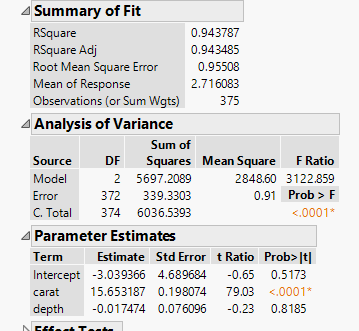
\includegraphics[scale=1.5]{carat_depth}}
\vspace{1cm}

\qparts{
\part[3] Using the JMP output, write the equation of the fitted linear relationship between carat, depth and price. \vspace{3cm}
\part[3] Using the fitted line, what do we suppose the price would be for a 1.07 carat and 62 depth diamond? \vspace{3cm}
\part[3] The actual price of a 1.07 carat with 62 depth diamond in the data is 11.434 thousand dollars. What is the residual for this specific diamond using the linear model? \vspace{3cm}
\part[3] For the linear relationship, find \(r\), the sample correlation coeffecient and \(R^2\), the coeffecient of determination. \vspace{3cm}
\part[3] Provide an estimate for $\sigma^2$. \vspace{3cm}
\part[3] Provide an estimate for the variance of the coefficient of *depth*. \vspace{3cm}
\part[5] Calculate and intepret the 95\% two-sided confidence interval for the coefficient of *depth*. \vspace{6cm}
\newpage
\part[10] Conduct a formal hypothesis test at the $\alpha = 0.05$ significance level to determine if there is significance relationship between price (y) and  **carat** $(x_1)$, holding depth constant. \\
\emph{Note: Write down all six steps for full credit.}
}

\newpage
\question

An arctic research station recently did a major overhaul to their server
system hardware and the technicians are checking to make sure that there
has been no loss in download speed. The previous download speed had an
average of 63.4 Mbps. A systems analyst took 10 readings on the download
speeds during the course of a day to check. Her results are below (in
Mbps):

\begin{center} 63.15, 62.85, 63.28, 63.03, 63.18, 62.91, 62.61, 62.98, 62.73, 63.03 \end{center}

The sample average is 62.98 and the sample variance is 0.043.

\qparts{
\part[5] Provide a 90\% confidence interval for the mean download speed. \vspace{2cm}
\part[5] Provide a 95\% lower confidence bound for the mean download speed. \vspace{2cm}
\part[10] Conduct a hypothesis test at the 95\% confidence level for the null hypothesis $\mu \ge 63.4$ against the alternative $\mu < 63.4$. Include your hypothesis statement, the choice of test statistic, the p-value, and your conclusion.
}

\newpage

\question A group of scientists are trying to understand the effects of
temperature on two O-ring designs for a rocket. By placing the O-ring
(attached to a valve) in a chamber and slowly lowering the chamber's
temperature, the scientists are able to record the temperature at which
the O-ring fails by monitoring when the valve begins to leak. After
testing 10 O-rings for each type, the scientists find the mean failure
temperature for the first O-ring design sample to be \(50\) K with a
sample variance of 10 and the mean failure temperature of the second
O-ring sample to be \(53\) K with a sample variance of \(20\). \qparts{
\part[4] Provide a 95\% confidence interval for the true failure temperature of the first O-ring design. \vspace{3cm}
\part[4] Provide a 95\% confidence interval for the true failure temperature of the second O-ring design. \vspace{3cm}
\part[10] Conduct a hypothesis test at the 90\% confidence level to see if the true failure temperature of the first sample is equal to that of second sample.  

} \newpage \question Let \(X\) be a normal random variable with a mean
of 5 and a varaince of 4 (i.e., \(X \sim N(5,4)\)) and let \(Z\) be a
random variable following a standard normal distribution. Find the
following probabilities (note: the attached standard normal probability
table may be helpful): \qparts{
   \part[2] $P(Z \le 1.5)$ \vspace{2cm}
   \part[2] $P(|Z| \ge 1.25)$ \vspace{2cm}
   \part[2] $P(1 \le X < 9)$ \vspace{2cm}
   \part[2] $P(|X| \le 5)$ \vspace{2cm}
}

\question

Suppose that \(X\) is a continuous random variable with probability
density function (pdf):
\[f(x) = \begin{cases} 0 &  x < 0 \\ 2 e^{-2x} &  x \ge 0 \end{cases}\]

\qparts{
 \part[3] Find F(x), the cumulative probability function. \vspace{3cm}
 \part[3] What is the probability that $X$ takes a value less than 1? \vspace{2cm}
 \part[3] What is the probability that $X$ takes a value greater than 2? \vspace{2cm}
}

\newpage

\question

Suppose that \(X\) is a discrete random variable with the following
probability function:
\[f(x) = \begin{cases} \dfrac{x^2}{c} & x = -3, -2, -1, 0, 1, 2, 3 \\ 0 & o.w \end{cases}\]

where \(c\) is a constant. \qparts{
   \part[4] Find the value of $c$ that makes $f(x)$ a valid probability function. \vspace{4cm}
   \part[3] Find $P(X \ge 2)$. \vspace{4cm}
   \part[3] Find $E(X)$.
}

\newpage

\question

Let \(X\) be a random variable with Binomial distribution
\(x\sim Binomial(n=10, p=0.2)\) and Y be a Normally distributed random
variable with mean \(\mu=1\) and variance \(\sigma^2=4\).

\qparts{
\part[2] Find the expected value of $2^{-1}X + 3Y -4$\vspace{3cm}
\part[4] Find the **standard deviation** of $3 X + 2^{-1}Y + 1/2$

}
		
	\end{questions}
	
\end{document}
